\documentclass[11pt]{article}
\usepackage[paper=letterpaper,margin=1in]{geometry}
\usepackage{mathtools}

\DeclarePairedDelimiter\ceil{\lceil}{\rceil}
\DeclarePairedDelimiter\floor{\lfloor}{\rfloor}
\usepackage[parfill]{parskip}
\usepackage{amsmath}
\usepackage{listings}
\DeclareFontShape{OT1}{cmtt}{bx}{n}{<5><6><7><8><9><10><10.95><12><14.4><17.28><20.74><24.88>cmttb10.95}{}
\usepackage{caption}
\usepackage{fancybox}
\usepackage[obeyspaces,spaces]{url}
\usepackage{graphicx}
\usepackage{wasysym}
\usepackage{fancyvrb}
\newcommand*{\vpointer}{\vcenter{\hbox{\scalebox{2}{\Huge\longrightarrow}}}}
\makeatletter
\newenvironment{CenteredBox}{% 
\begin{Sbox}}{% Save the content in a box
\end{Sbox}\centerline{\parbox{\wd\@Sbox}{\TheSbox}}}% And output it centered
\makeatother
\usepackage{tikz}
\def\CC{{C\nolinebreak[4]\hspace{-.05em}\raisebox{.4ex}{\tiny\bf ++ }}}
\usepackage[
backend=biber,
citestyle=alphabetic,
style=alphabetic,
sorting=ynt
]{biblatex}
\lstset { %
    escapeinside={(*@}{@*)},
    language=C++,
    basicstyle=\ttfamily,% basic font setting
}
\addbibresource{sample.bib}
\DeclareUrlCommand\class{%
  \renewcommand{\UrlBigBreaks}{\do\.}%
  \renewcommand{\UrlBreaks}{\do\.}%
  }
\DeclareUrlCommand\filedir{%
  \renewcommand{\UrlBigBreaks}{\do\\}%
  \renewcommand{\UrlBreaks}{\do\\}%
  }
\DeclareUrlCommand\method{%
  \renewcommand{\UrlBigBreaks}{}%
  \renewcommand{\UrlBreaks}{}%
  }
\definecolor{mygrey}{rgb}{.85,.85,.85}

\begin{document}
\thispagestyle{empty}
\title{Branch and Bound: Assignment Problem \\
\large Assignment 505 \\
CS 310}
\date{May 4, 2017}
\author{Cameron Moberg}
\maketitle
 
Branch and bound is a algorithm design for optimization, in this case an optimization for combinatorial optimization. In this 

\section{Unmodified Performance}
\subsection{Minimum Considers}
In order to find the input that causes the least amount of considering lines, we must examine the code and work backwards. The code calculates the lower bound for the first level of input, finds the node with lowest bound, and repeats that process for the next level with the added constraint of the inability to use the column that was just used. An example input is shown below, where bold means that the job assignment has been chosen or is being considered.
\begin{Verbatim}[commandchars=\\\{\},codes={\catcode`\$=3\catcode`_=8}]
\textbf{1 \!2 2 2} 	     \textbf{1} 2 2 2 	     \,\textbf{1} 2 2 2	     \textbf{1} 2 2 2
2 1 2 2 	     2 \textbf{1 2 2} 	     2 \textbf{1} 2 2 	    2 \textbf{1} 2 2
2 2 1 2 $\xrightarrow{\makebox[2cm]{}}$  2 2 1 2 $\xrightarrow{\makebox[2cm]{}}$  2 2 \textbf{1 2} $\xrightarrow{\makebox[2cm]{}}$ 2 2 \textbf{1} 2
2 2 2 1	      2 2 2 1 	     \,2 2 2 1	     \,2 2 2 \textbf{1}
\end{Verbatim}
\raisebox{2ex}{\textit{\tiny{Consider level 1 \kern 20ex Select 1, Consider level 2 \kern 15ex Select 1, Consider level 3 \kern 15ex Select 1, Consider level 4}}} \\
Now, because of the way the code is implemented, once the solution is found, it will not end until the priority queue is empty, causing unneeded considers in this case.
\subsection{Maximum Discards}
Much like previously, we must examine the code and work backwards to find a least optimal input that discards the greatest amount of nodes. In order to achieve the greatest number of discards, the algorithm must generate every possible permutation ($n!$ of them) before finding a solution. This occurs when every single value is the same, e.g. \\

\begin{CenteredBox}
  \begin{lstlisting}
1 1 1 1
1 1 1 1
1 1 1 1
1 1 1 1
  \end{lstlisting}
\end{CenteredBox}

This is because when it considers the very first level, it adds them all to the priority queue, and because this priority queue's comparator is implemented to keep order, the nodes keep their order. Since all of the nodes have the same lower bound, the program cannot rule any out, and will generate every permutation until it gets to the bottom level, where it will find a solution.

\subsection{Double Best Solution}
The goal was to find an input that found ``two best solutions''. However, upon closer inspection it does not appear possible to have an input that finds two best solutions. When we take a look at the code, we see that the program only finds a best solution on the bottom level (line 127). At every step the program chooses the most promising node, the one with the smallest lower bound, and it uses strictly less than when determining the best solution (lines 129, 149), so when it finds the first solution, it will be the only solution.

\section{Increasing Efficiency}
There are ways to increase the efficiency of this program (no offense) by taking advantage of what we saw when finding maximum discards, minimum considers, and multiple solutions. To decrease basic operations we must first determine what the basic operations is, and we chose the if statement in the  
\texttt{calculate\_lower\_bound()} method on line 62 since it's computationally expensive and occurs most frequently.

Overall, there were three things changed to improve efficiency.
\begin{enumerate}
\item Quickly calculate a baseline lower bound
\item Stop after finding a solution
\item Make calculating lower bound more efficient
\end{enumerate}

\subsection{Calculating a Baseline Lower Bound}
In the unmodified code on line 118 there is the line
\begin{lstlisting}[numbers=left, backgroundcolor = \color{mygrey}, language=C++, basicstyle=\footnotesize\ttfamily,firstnumber=118]
uint best_solution = UINT_MAX;
\end{lstlisting}

To increase efficiency we replaced that line with the below code in the modified file.
\lstinputlisting[backgroundcolor = \color{mygrey},language=C++, firstline=120,lastline=125,numbers=left,basicstyle=\footnotesize\ttfamily,firstnumber=120]{moberg_c_505.cpp}
This sets a baseline \texttt{best\_solution} which could potentially cut down on the number of lower bounds needed to calculate depending on the input and arrangement of numbers. When using this method on an input that are all the same number, as seen above, the program cuts down from 256 basic operations to only 64 in a 4 by 4 input.

\subsection{Stop After Solution Found}
As previously mentioned, when the program finds a solution it is the most optimal, meaning there is no need to continue checking the priority queue. On line 138, putting a simple \texttt{break;} statement in the loop allows the algorithm to potentially end much earlier than it was in the unmodified version, leading to less basic operations.

\subsection{Reinventing the Wheel}
\clearpage

To see the efficiency we ran four different programsL:
\begin{center}
    % GNUPLOT: LaTeX picture with Postscript
\begingroup
  \makeatletter
  \providecommand\color[2][]{%
    \GenericError{(gnuplot) \space\space\space\@spaces}{%
      Package color not loaded in conjunction with
      terminal option `colourtext'%
    }{See the gnuplot documentation for explanation.%
    }{Either use 'blacktext' in gnuplot or load the package
      color.sty in LaTeX.}%
    \renewcommand\color[2][]{}%
  }%
  \providecommand\includegraphics[2][]{%
    \GenericError{(gnuplot) \space\space\space\@spaces}{%
      Package graphicx or graphics not loaded%
    }{See the gnuplot documentation for explanation.%
    }{The gnuplot epslatex terminal needs graphicx.sty or graphics.sty.}%
    \renewcommand\includegraphics[2][]{}%
  }%
  \providecommand\rotatebox[2]{#2}%
  \@ifundefined{ifGPcolor}{%
    \newif\ifGPcolor
    \GPcolorfalse
  }{}%
  \@ifundefined{ifGPblacktext}{%
    \newif\ifGPblacktext
    \GPblacktexttrue
  }{}%
  % define a \g@addto@macro without @ in the name:
  \let\gplgaddtomacro\g@addto@macro
  % define empty templates for all commands taking text:
  \gdef\gplbacktext{}%
  \gdef\gplfronttext{}%
  \makeatother
  \ifGPblacktext
    % no textcolor at all
    \def\colorrgb#1{}%
    \def\colorgray#1{}%
  \else
    % gray or color?
    \ifGPcolor
      \def\colorrgb#1{\color[rgb]{#1}}%
      \def\colorgray#1{\color[gray]{#1}}%
      \expandafter\def\csname LTw\endcsname{\color{white}}%
      \expandafter\def\csname LTb\endcsname{\color{black}}%
      \expandafter\def\csname LTa\endcsname{\color{black}}%
      \expandafter\def\csname LT0\endcsname{\color[rgb]{1,0,0}}%
      \expandafter\def\csname LT1\endcsname{\color[rgb]{0,1,0}}%
      \expandafter\def\csname LT2\endcsname{\color[rgb]{0,0,1}}%
      \expandafter\def\csname LT3\endcsname{\color[rgb]{1,0,1}}%
      \expandafter\def\csname LT4\endcsname{\color[rgb]{0,1,1}}%
      \expandafter\def\csname LT5\endcsname{\color[rgb]{1,1,0}}%
      \expandafter\def\csname LT6\endcsname{\color[rgb]{0,0,0}}%
      \expandafter\def\csname LT7\endcsname{\color[rgb]{1,0.3,0}}%
      \expandafter\def\csname LT8\endcsname{\color[rgb]{0.5,0.5,0.5}}%
    \else
      % gray
      \def\colorrgb#1{\color{black}}%
      \def\colorgray#1{\color[gray]{#1}}%
      \expandafter\def\csname LTw\endcsname{\color{white}}%
      \expandafter\def\csname LTb\endcsname{\color{black}}%
      \expandafter\def\csname LTa\endcsname{\color{black}}%
      \expandafter\def\csname LT0\endcsname{\color{black}}%
      \expandafter\def\csname LT1\endcsname{\color{black}}%
      \expandafter\def\csname LT2\endcsname{\color{black}}%
      \expandafter\def\csname LT3\endcsname{\color{black}}%
      \expandafter\def\csname LT4\endcsname{\color{black}}%
      \expandafter\def\csname LT5\endcsname{\color{black}}%
      \expandafter\def\csname LT6\endcsname{\color{black}}%
      \expandafter\def\csname LT7\endcsname{\color{black}}%
      \expandafter\def\csname LT8\endcsname{\color{black}}%
    \fi
  \fi
    \setlength{\unitlength}{0.0500bp}%
    \ifx\gptboxheight\undefined%
      \newlength{\gptboxheight}%
      \newlength{\gptboxwidth}%
      \newsavebox{\gptboxtext}%
    \fi%
    \setlength{\fboxrule}{0.5pt}%
    \setlength{\fboxsep}{1pt}%
\begin{picture}(7200.00,5040.00)%
    \gplgaddtomacro\gplbacktext{%
      \csname LTb\endcsname%
      \put(814,704){\makebox(0,0)[r]{\strut{}$0$}}%
      \csname LTb\endcsname%
      \put(814,1439){\makebox(0,0)[r]{\strut{}$50$}}%
      \csname LTb\endcsname%
      \put(814,2174){\makebox(0,0)[r]{\strut{}$100$}}%
      \csname LTb\endcsname%
      \put(814,2909){\makebox(0,0)[r]{\strut{}$150$}}%
      \csname LTb\endcsname%
      \put(814,3644){\makebox(0,0)[r]{\strut{}$200$}}%
      \csname LTb\endcsname%
      \put(814,4379){\makebox(0,0)[r]{\strut{}$250$}}%
      \put(2117,484){\makebox(0,0){\strut{}Original}}%
      \put(3289,484){\makebox(0,0){\strut{}Baseline}}%
      \put(4460,484){\makebox(0,0){\strut{}Break}}%
      \put(5632,484){\makebox(0,0){\strut{}Both}}%
    }%
    \gplgaddtomacro\gplfronttext{%
      \csname LTb\endcsname%
      \put(176,2541){\rotatebox{-270}{\makebox(0,0){\strut{}Basic Operations}}}%
      \put(3874,154){\makebox(0,0){\strut{}Type of Modification}}%
      \put(3874,4709){\makebox(0,0){\strut{}Average Basic Operations by Modification with 4x4 Input Size}}%
    }%
    \gplbacktext
    \put(0,0){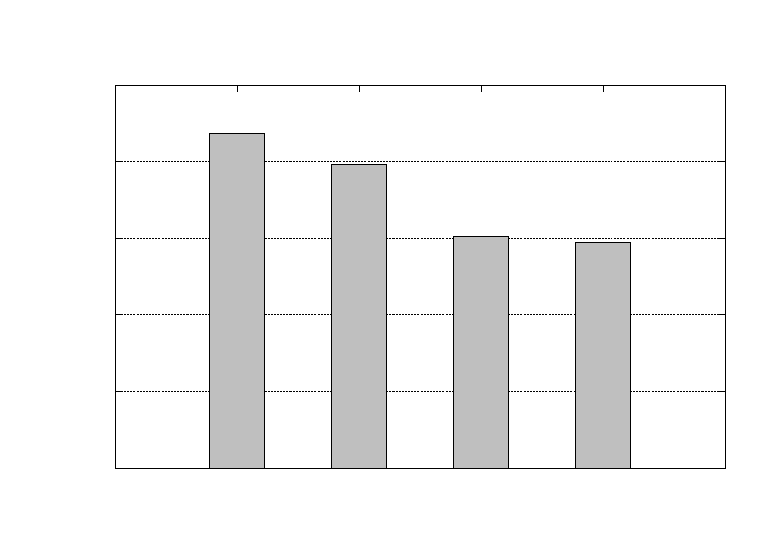
\includegraphics{bar}}%
    \gplfronttext
  \end{picture}%
\endgroup

\end{center}
\end{document}